\documentclass{article}
\author{Maria Alejandra Arias Jaimes}
\usepackage[utf8]{inputenc}
\date{20 de julio de 2017}
\title{Métodos Computacionales. Tarea 3}
\usepackage[utf8]{inputenc}
\usepackage{amsmath, amssymb, graphicx}
\usepackage[utf8]{inputenc}

\frenchspacing

\newcommand{\JournalIssue}[1]{%
                \hfill \textsc{20 de Julio de 2017}
                \par \normalsize \normalfont}

\newcommand{\JournalName}[1]{%
                \begin{center}
                        \Huge \usefont{T1}{m}{n}
                        #1%
                \end{center}
                \par \normalsize \normalfont}
\newcommand{\NewsAuthor}[1]{%
                        \hfill \textsc{Maria Alejandra Arias Jaimes 201415329}
                        \par \normalsize \normalfont}

\begin{document}
\JournalIssue{1}
\NewsAuthor{}
\JournalName{ TTarea 3 Métodos Computacionales}

\section{Propagación Onda}

La simulación se obtuvo al resolver la ecuación de onda bidimensional.

\begin{figure}[h!]
\centering
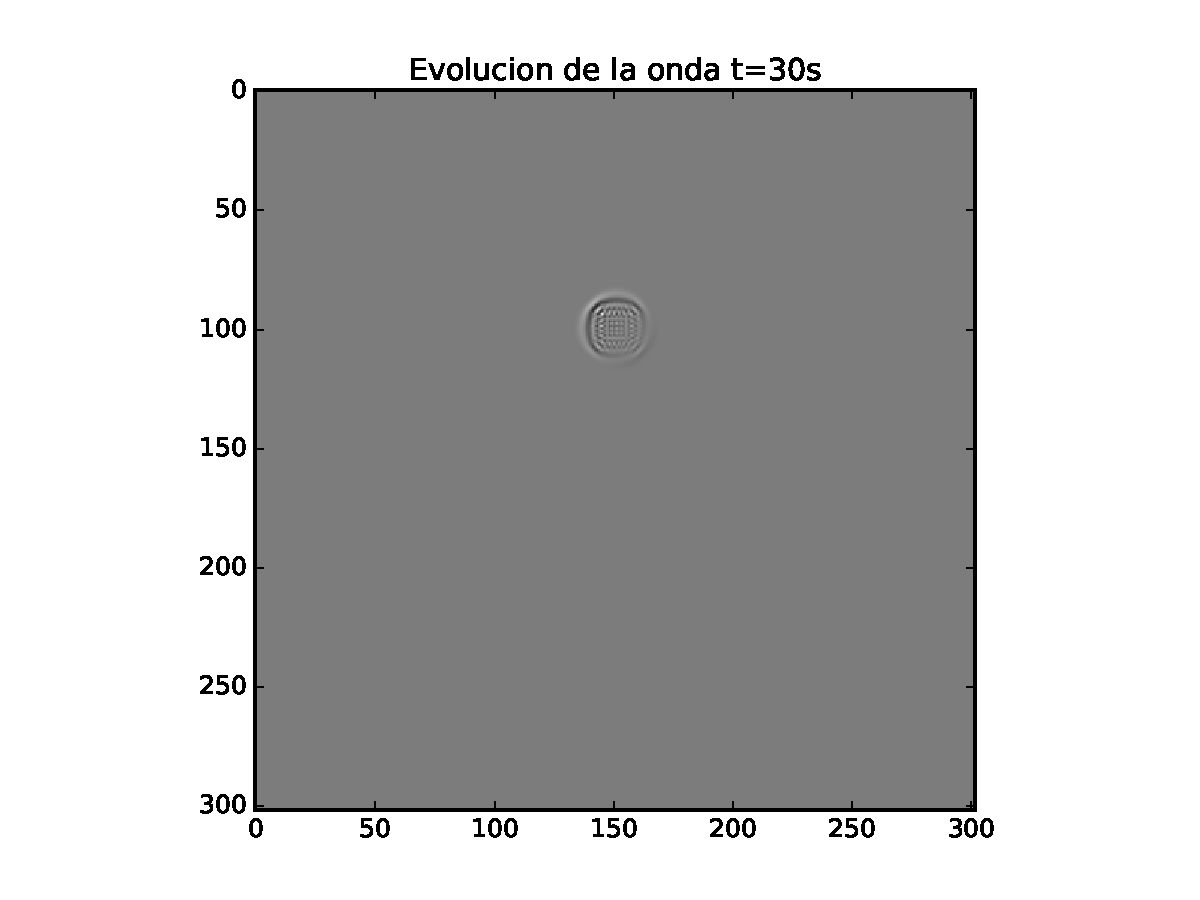
\includegraphics[width=0.7\textwidth]{Onda_30.png}
\caption{Propagacion de la onda en t=30s.}
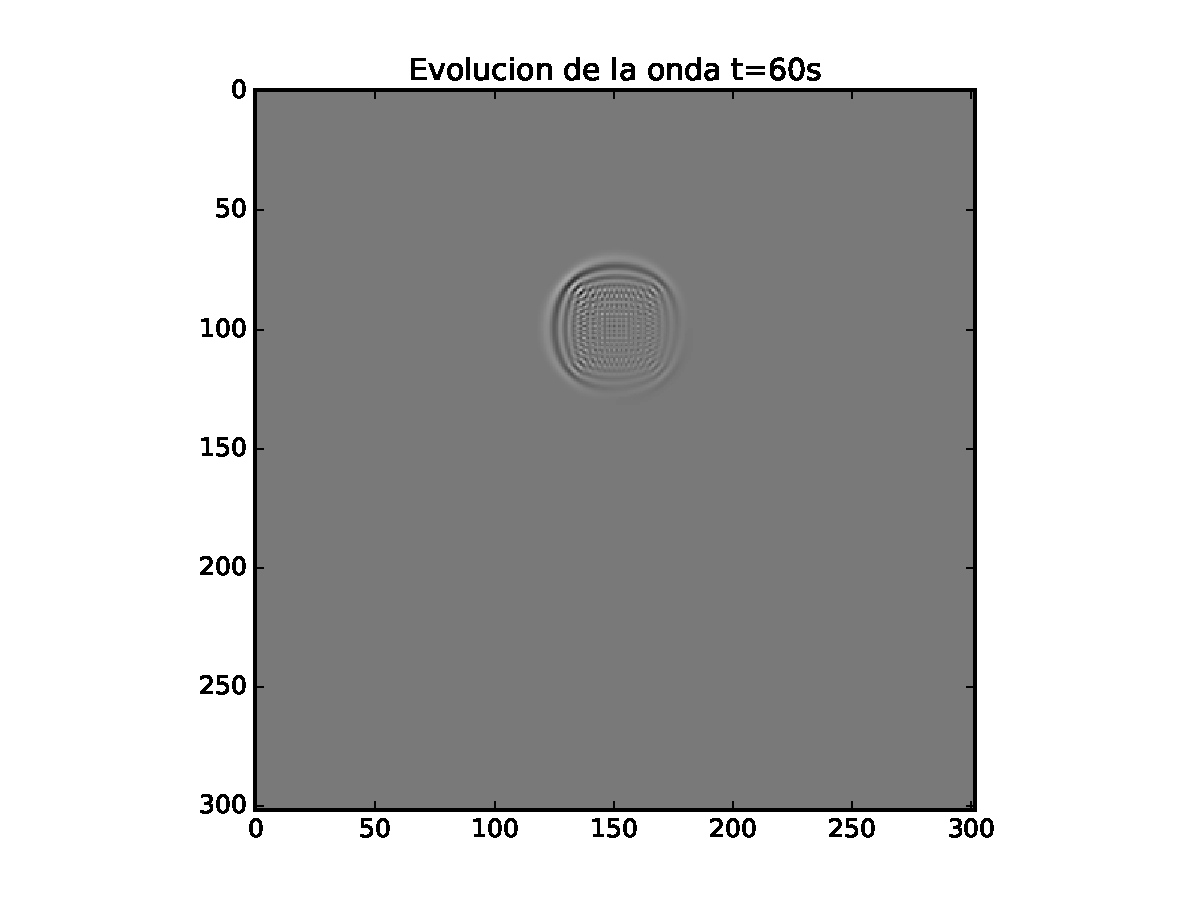
\includegraphics[width=0.7\textwidth]{Onda_60.png}
\caption{Propagacion de la onda en t=60s.}
\end{figure}

 
\section{Planetas}



\begin{figure}[h!]
\centering
\includegraphics[width=0.7\textwidth]{Orbitas.png}
\caption{Esto no es de la orbita, la incluí la poder correr el makefile}

\end{figure}

\end{document}

